%!TEX root = ../terrainbook.tex
% chktex-file 46

\setchapterpreamble[u]{\margintoc}
\graphicspath{{gdem/figs/}}


\chapter{Global digital elevation models}% or global terrains
\label{chap:gdem}

We define as ``global digital elevation models'' (or global terrains) the datasets that cover (most of) the Earth (gDEM below).%
\index{global DEM}
Those datasets require different acquisition methods from local datasets, since flying an airplane or performing local surveys at the scale of the Earth has not been done as it would prohibitively expensive.
The acquisition instruments used must be \emph{space-borne}, \ie\ mounted on a satellite for instance.
Notice that the orbit of some satellites makes them technically non-global, but that we still refer to their datasets as global since they have a wide coverage, just restricted to certain latitudes.

It cannot be understated that before the introduction of gDEMs (in 2001), we had no way of knowing the elevation for most of the Earth.
Indeed, looking at the map in Figure~\ref{fig:dem_coverage}, we see that local elevation datasets are limited to developed countries.

\begin{figure}
  \centering
  \caption{OpenTopography coverage + European datasets.}%
  \label{fig:dem_coverage}
\end{figure}

Global DEMs thus enabled \emph{global} environmental studies, such as geological studies, hydrological modelling, ecosystems dynamics, and their ubiquitous use in flood modelling (see Chapter~\ref{chap:runoff}).
However, gDEMS have several properties and characteristics that apply only to them, and we report in this chapter on the main ones.

% a few examples are the detection geological structures, the analysis of tectonic evolution, flood modelling, and the understanding of volcanic processes.

% We first describe global acquisition techniques, then we discuss the properties (and errors and biases, etc.) that the datasets collected will have,

%%%%%%%%%%%%%%%%%%%%
%
\section[Acquisition of global data]{Acquisition of global elevation data}

The acquisition of gDEMs requires the use of a sensor mounted on a satellite.
The three most used instruments to collect elevation information are:

\begin{enumerate}
  \item Photogrammetry from optical satellite images
  \item Interferometric synthetic-aperture radar (InSAR)
  \item Spaceborne lidar
\end{enumerate}

%%%
\subsection{InSAR}

The first gDEM (SRTM v1) was measured with InSAR in 2000, aboard the Space Shuttle Endeavour.
As InSAR requires two images of the same area for stereoscopy to derive a DEM, the Shuttle was equipped with two antennas, one in the payload bay, and one a mast extending \qty{60}{m} from the Shuttle.

Similarly, the TerraSAR-X satellite was joined by TanDEM-X in 2010, a twin satellite orbiting only a few hundred meters(!) away, to generate InSAR data in a single pass.

See Section~\ref{sec:insar}.

%%%
\subsection{Photogrammetry from high-resolution satellite images}

See Section~\ref{sec:photogrammetry}.




%%%
\subsection{Spaceborne lidar (ICESat-2 + GEDI)}
Spaceborne lidar is a relatively new technique, and has not yet been used to produce a gDEM.
We still include it here because it enables \emph{terrain} elevation measurements globally.

Lidar was first used in space on the Apollo missions, and with further technological developments, it has been used extensively from the 1990s onwards.
For example, Mercury, Mars, near-Earth asteroids, and lately again the moon have been scanned using lidar.
Earth surface elevation lidar measurements have also been developed, often flown on the Space Shuttles.
ICESat was the first Earth-based lidar satellite, launched in 2003, with the primary goal of ice sheet monitoring.
It had an elevation accuracy of several cm and was operational for five years.
Most recently, NASA launched in 2018 two missions measure the elevation of the Earth globally with lidar instruments:

\begin{itemize}
  \item \textbf{ICESat-2}
        \marginnote{\url{https://icesat-2.gsfc.nasa.gov/}}
        (Ice, Cloud, and Land Elevation Satellite-2) is in a low Earth and polar orbit to investigate ice sheets, it covers the Earth between \ang{-88} and \ang{88} latitude.
        Its instrument to measure altimetry is called \emph{Advanced Topographic Laser Altimeter System} (ATLAS).
        Apart from terrain retrieval, ICESat-2 also measures the surface, such as canopy height, and has many other applications such as measuring bathymetry and estimating biomass.
  \item \textbf{GEDI}
        \marginnote{\url{https://gedi.umd.edu/}}
        (Global Ecosystem Dynamics Investigation) is attached to the international space station (ISS) and its main goal is to investigate global ecosystems.
        It does not have global coverage since it collects measurements only between \ang{51.6} N and \ang{51.6} S.
        GEDI has been combined with TanDEM-X data to produce biomass estimates and with Landsat imagery to produce a global canopy height map.
\end{itemize}
\begin{figure*}
  \centering
  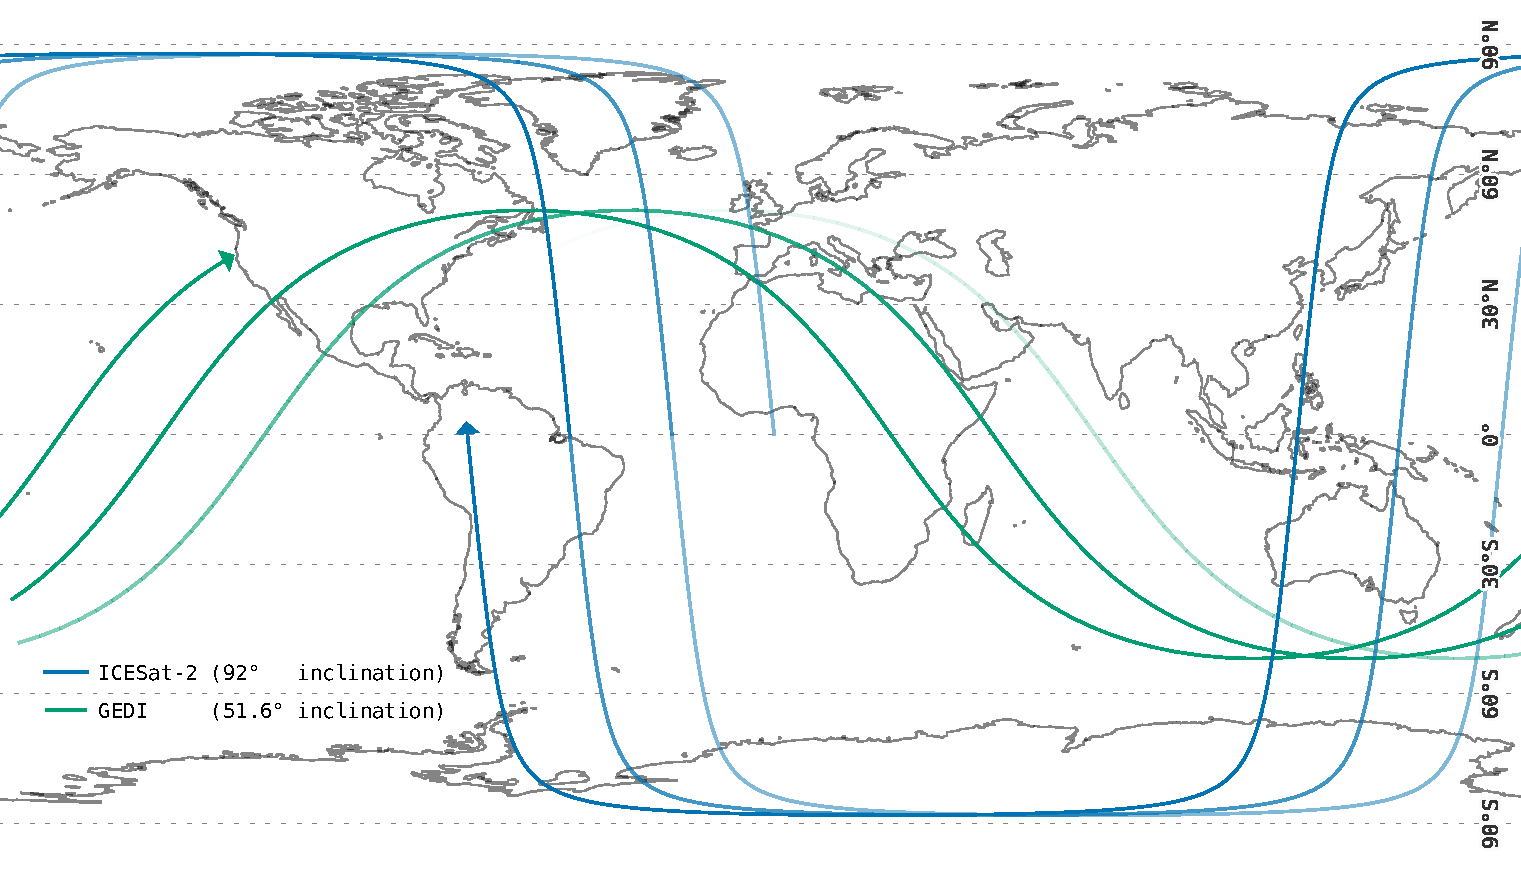
\includegraphics[width=\linewidth]{orbit}
  \caption{Ground tracks for three successive orbits of ICESat-2 and GEDI. The satellite is a represented by a triangle and past orbits fade out. Note the increased density of ground tracks at the latitude of inclination, as well as the lack of coverage beyond \ang{51.6}~latitude for GEDI.}%
  \labfig{fig:orbit}
\end{figure*}

%

The characteristics of both missions are summarised in Table~\ref{tab:lidarcomparison}
\begin{table*}
  \sisetup{detect-weight=true,detect-inline-weight=math}
  \caption{Key characteristics of GEDI and ICESat-2 missions in comparison with a typical airborne lidar mission.}
  \centering
  \begin{tabular}{llll}
    \toprule
                           & ICESat-2                             & GEDI                                   & airborne lidar   \\
    \midrule
    \ type                 & discrete photon                      & full waveform                          & either           \\
    \ objective            & cryosphere monitoring                & Ecosystems                             & -                \\
    \ duration             & 2019-2022                            & 2019-2021                              & single flight(s) \\
    \ orbit inclination    & \ang{92}                             & \ang{51.6}                             & NA               \\
    \ laser pulse power    & \qty{175}{{\mu}J}/\qty{45}{{\mu}J}   & \qty{10000}{{\mu}J}/\qty{5000}{{\mu}J} & NA               \\
    \ elevation            & \qty{\pm480}{km}                     & \qty{\pm420}{km}                       & \qty{0.5}{km}    \\
    \ beam footprint       & \qty{17}{m}                          & \qty{23}{m}                            & \qty{0.05}{m}    \\
    \ along track spacing  & \qty{0.7}{m}                         & \qty{70}{m}                            & \qty{0.1}{m}     \\
    \ across track spacing & \qty{3}{km}/\qty{90}{m} between pair & \qty{0.6}{km}                          & \qty{0.1}{m}     \\
    \ swath width          & \qty{6.6}{km}                        & \qty{4.2}{km}                          & \qty{1}{km}      \\
    \ beam frequency       & \qty{512}{nm} (green)                & \qty{1064}{nm} (near-infrared)         & either           \\
    \ \# beams             & 6 (in 3 pairs)                       & 8                                      & 1                \\
    \bottomrule
  \end{tabular}%
  \label{tab:lidarcomparison}
\end{table*}

%

\begin{figure}
  \centering
  \includegraphics[width=0.8\linewidth]{tracks}
  \caption{Filtered ICESat-2 and GEDI points from a single granule each at the 47th latitude, demonstrating the beam patterns.
    Note that ICESat-2 has a smaller beam footprint and a much higher pulse repetition, but a more uneven spatial coverage than GEDI\@.
    The gaps between data here will decrease by using multiple granules, but will never disappear completely.}%
  \label{fig:beams}
\end{figure}

ICESat-2 lasers split into six beams, divided into three pairs, each pair \qty{90}{m} apart and the pairs \qty{3.3}{km} apart, for a total swath width of \qty{6.6}{km}.
Along-track, it can measure each \qty{0.7}{m}, while its beam footprint is \qty{\pm17}{m}, so each measurement overlaps.
GEDI sensor has eight beams, each \qty{600}{m} apart, for a total swath width of \qty{4.2}{km}.
GEDI measures a point every \qty{70}{m} along-track, with a beam footprint of \qty{23}{m}.
Furthermore, whereas GEDI employs a full-waveform laser at a typical near-infrared wavelength of \qty{1064}{nm}, ICESat-2 employs a single-photon LiDAR at a bathymetric ``green'' wavelength of \qty{512}{nm}.

%%%
\paragraph{Comparison to typical airbone lidar.}
These space borne lasers also differ considerably from airborne lasers, most notably so in their platform, resulting in significant differences in beam footprint and ground coverage.
The altitude increase results in a wider beam footprint, from \qty{\sim0.5}{m} (at \qty{500}{m}) for airborne platforms to \qty{\sim15}{m} for space platforms.
Although much wider, it is a small increase compared to the increase in altitude, going from \qty{0.5}{km} to \qty{480}{km}.
A comparison is given in Table~\ref{tab:lidarcomparison}.
Airborne LiDAR often focuses on maximizing coverage (\unit{points/m^2}) of smaller areas, whereas the coverage for space lasers is the ground track of the satellite.
While both ICESat-2 and GEDI employ instruments with multiple (split) laser beams, including the ability to point the laser away from the ground track, all to maximize coverage, this still results in very sparse and uneven coverage as shown in Figure~\ref{fig:beams}.



%%%%%%%%%%%%%%%%%%%%
%
\section[Specific characteristics]{Specific characteristics of gDEMs}

%%
\paragraph{Global often means near-global}

The data collected depend on the orbit of the satellite.
Some satellites have a polar orbit and can therefore completely measure the Earth (ICESat-2 is one example, see~\reffig{fig:orbit}), while some will cover only certain latitudes (\eg\ GEDI, see~\reffig{fig:orbit}).
Similarly, while the Tandem-X mission produced a DEM with a global coverage, the SRTM DEM was measured from the Space Shuttle and only covered up to \qty{60}{\degree} latitude.


%%
\paragraph{Vertical datums}
% Do students know about geoids? If not, explain it here, ellipsoid vs geoid.
Global DEMs are often vertically referenced to the geoid, specifically EGM96 for SRTM and EGM2008 (EPSG:3855) for CopernicusDEM.
There's a small difference---generally less than half a metre---between these versions of the EGM geoid.

% MSS = Geoid + MDT
Note that the geoid is not the same as Mean Sea Level (MSL), as it does not take into account the dynamic effects of temperature and currents.
Depending on the location, the difference between the geoid and MSL can be up to 1.5 metres.

%%
\paragraph{Format}  % include resolution
The format of DEMs has historically been defined by the military, which are still used by many government agencies.
There is the Digital Terrain Elevation Data (DTED) format, developed in the 1970s, which stores elevation in integers (saying something about the accuracy back then).
It specifies several possible \emph{levels} in terms of resolution (in arcseconds), from level 0 at \qty{\pm1}{km} to level 2 at \qty{30}{m}.
More recently, in 2016, the Defense Gridded Elevation Data (DGED) has been defined, specifiying more levels to higher resolutions and allowing for geotiffs.
It also defines the structure and specific tiling of the data at higher latitudes, as resolutions in arcseconds become smaller near the poles.

Datasets such as SRTM and derived NASADEM will provide data as .hgt (height) files, which are not even a format, but are simply a binary file with the elevation data, with the geographic extent to be derived from the filename.
GDAL can read these files.


%% Accuracy?
\paragraph{Errors}
As with any measurements taken, gDEMs contain errors, or outliers.
SRTM for example, contains a lot of noise, and has (diagonal) striping artefacts.
CopernicusDEM suffers from multipath errors in urban areas, which lead to small pits in the DEM.

Most gDEMS suffer from voids in steep terrain, as peaks can occlude valleys below (shadow effect).
%%\paragraph{void filling: \url{https://en.wikipedia.org/wiki/Shuttle_Radar_Topography_Mission#Void-filled_SRTM_datasets}
These voids are often filled in not (only) by interpolation, but by other gDEMS, as they measured the same area from a different angle.


Global DEM products are often accompanied by a quality layer, which indicates where data has been void-filled.
Similarly, error masks with the calculated instrument error and water masks are often provided alongside the elevation data.
% Something about vertical accuracy, it getting better.

%%
% \paragraph{integration with sea-level datasets}


%%
% \paragraph{accuracy affected by slope (most image-based products)}


%%
\paragraph{DSM (more than DTM)}
In contrast to local DEMs, which are often provided as either a classified pointcloud, or as separate raster DSM and DTMs, gDEMs should be classified as DSMs.
The current measurement techniques will measure the top of canopy and buildings, and not the ground below.
This is the largest source of error in gDEMS, and can considerably limit the applicability of the data.

Several attempts have been made to correct gDEMS for vegetation and buildings, leading to what we denote as a pseudo DTM ('DTM).
While these methods improve the accuracy of gDEMs considerably, they are not perfect, and results are still far removed from a local DTM.

%%%%%%%%%%%%%%%%%%%%
%
\section[Most common products]{Most common products available}

An overview of the most common gDEMS are given in Figure~\ref{fig:gdem_inheritance}.
Note that all these products differ considerably in terms of coverage, resolution, accuracy and licensing.
Even the same product can have different versions, with different resolutions and licenses.

For example, SRTM is freely available, including its derived NASADEM, and was first introduced at \qty{90}{m}, with subsequent versions at \qty{30}{m}.
Tandem-X, and its derived WorldDEM, is a commercial product, with a resolution of \qty{\pm12}{m}.
WorldDEM-NEO, a newer version of WorldDEM with more Tandem-X data, even has a resolution of \qty{\pm5}{m}.
CopernicusDEM is a resampled WorldDEM---bought with your taxpayer money by ESA and freely distributed---at \qty{30}{m} resolution.
The pseudo DTM FABDEM, while derived from the free CopernicusDEM, is only free for research purposes.

Similarly, while ALOS World3D is freely available at \qty{30}{m}, it also comes in a commercial version at \qty{5}{m} resolution.
There is even a \qty{0.5}{m} commercial version, based on multiple optical satellites, available on request.

% We list only the ones available as open-access?
% For instance AW3D is also available as 5m-grid, but €€€.

% Maybe we should make our own table with paid products too? Like that table: \url{https://github.com/DahnJ/Awesome-DEM#summary}
% I find it interesting to know that some products are not free, and way better

% TODO: remake the inheritance fig
\begin{figure}
  \centering
  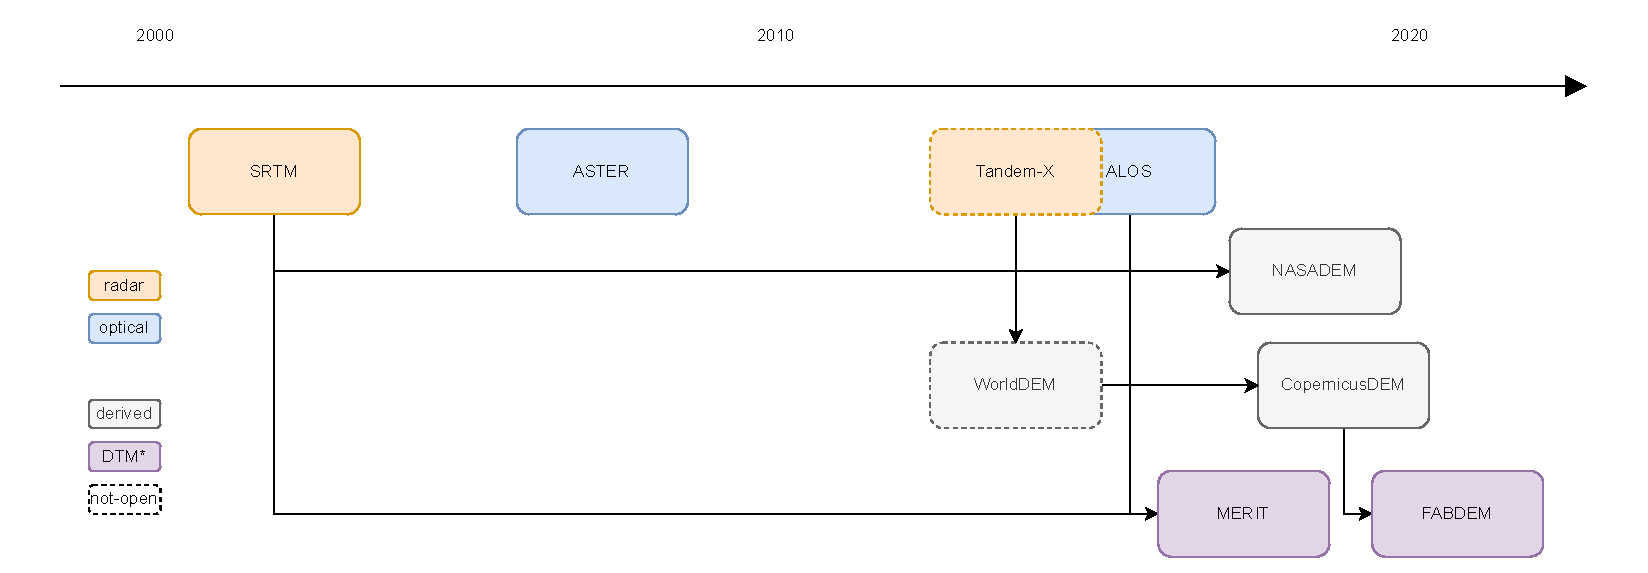
\includegraphics[width=\linewidth]{dems_overview}
  \caption{An overview of current gDEMs}%
  \labfig{fig:gdem_inheritance}
\end{figure}

% TODO: Make into table with resolution(s) (paid-free) and maybe license(s) (research-non-commercial)
\begin{itemize}
  \item ASTER
  \item ALOS World 3D
  \item STRM
  \item NASADEM
  \item CopernicusDEM
  \item MERIT
  \item FABDEM
\end{itemize}

% A few words about fusion? [Okolie22] has very long review.

% These subfigures (images are the same size) have a horizontal shift in the book?
\begin{figure}
  \centering
  \begin{subfigure}{0.45\linewidth}
    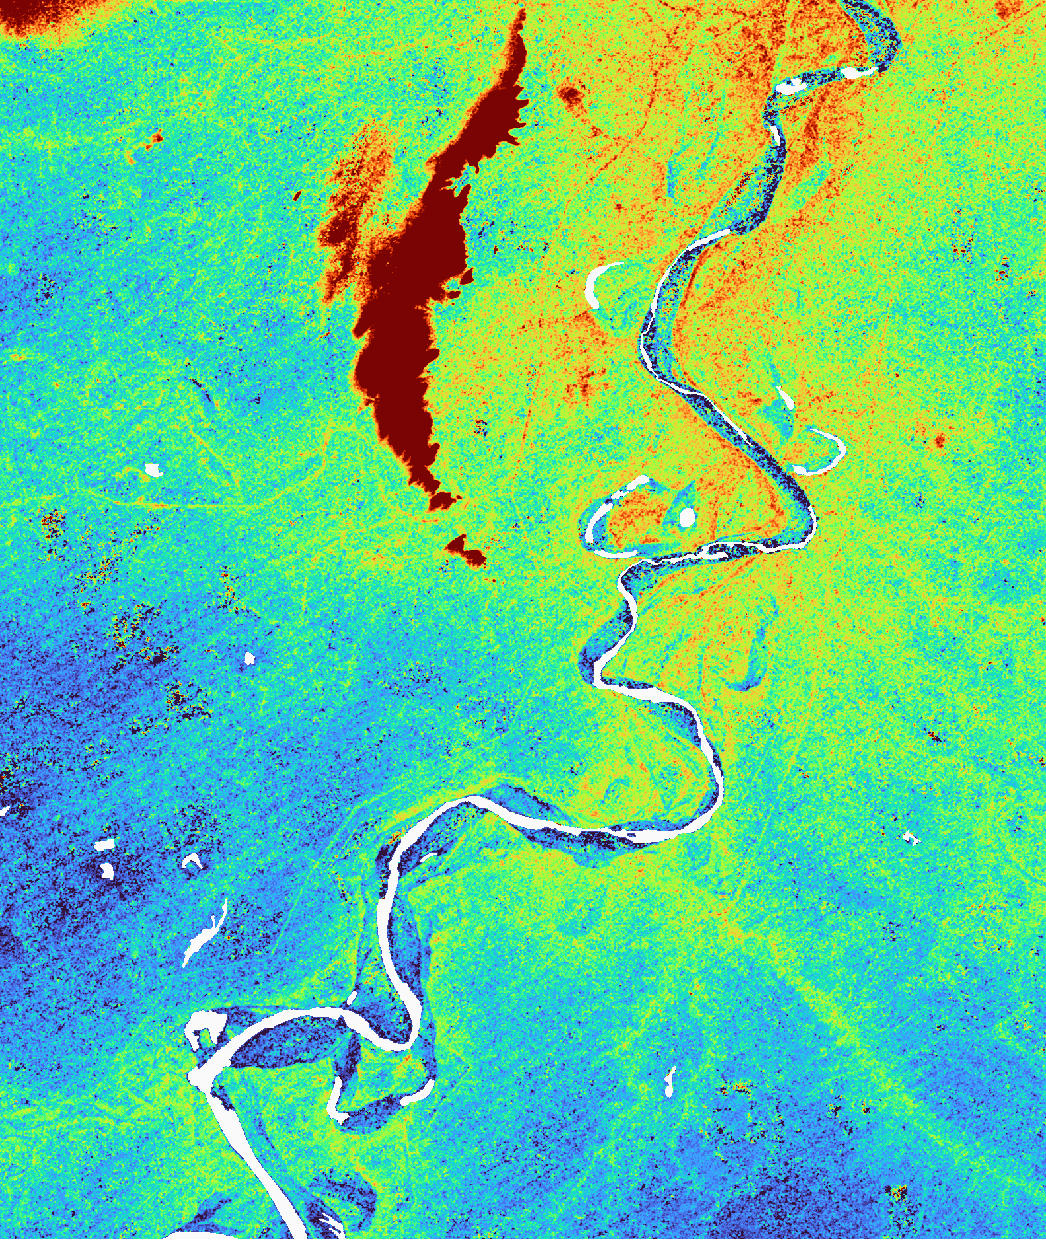
\includegraphics[width=\linewidth]{nasadem.png}
    \caption{NASADEM}
    \label{fig:nasadem}
  \end{subfigure}
  \hfill
  \begin{subfigure}{0.45\linewidth}
    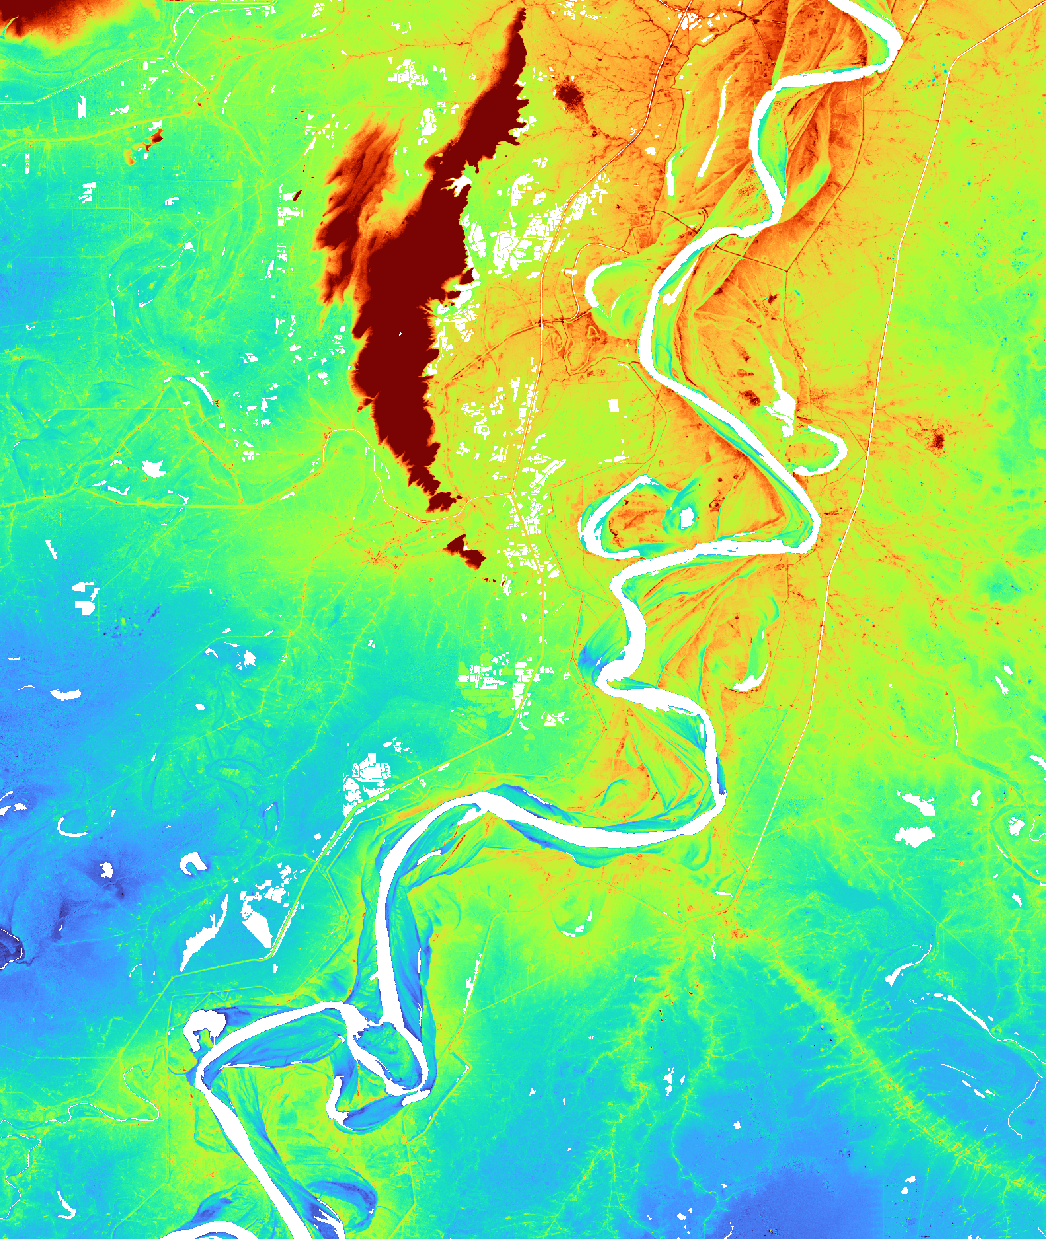
\includegraphics[width=\linewidth]{copernicusdem.png}
    \caption{CopernicusDEM}
    \label{fig:copernicusdem}
  \end{subfigure}
  \caption{NASADEM and CopernicusDEM compared for the same area; Indus delta, Pakistan.
    Note the striped noise in NASADEM, and how CopernicusDEM has more detail.
    There is $\pm$twelve years between these images.}%
  \label{fig:three graphs}
\end{figure}


%%%%%%%%%%%%%%%%%%%%
%
\section{Notes \& comments}

\citet{Yang11} provide a detailed list of applications where gDEMs (SRTM, but when the paper was written (2011) SRTM was still the main product available globally) are necessary as input.

Arguably the best place to download DEMs (gDEMS, local ones, lidar datasets, etc.) is OpenTopography (\url{https://opentopography.org}).
Otherwise each gDEM has its own download portal, with its own registration systems and its specific ways of searching and downloading the data.




%%%%%%%%%%%%%%%%%%%%
%
\section{Exercises}

\begin{enumerate}
  \item What is what?
\end{enumerate}
